\documentclass[arial,11pt]{article}
%\documentclass[11pt]{nih}
\usepackage[dvips]{graphicx}
\usepackage[colorlinks=true,linkcolor=black]{hyperref}
\usepackage{amssymb}
%\usepackage{graphicx}
%\usepackage{longtable}
\usepackage{epsfig}
%\usepackage{overcite}
\usepackage[usenames]{color}

\renewcommand{\rmdefault}{phv} % Arial
\renewcommand{\sfdefault}{phv} % Arial
\renewcommand{\thesection}{\Alph{section}}
\pagestyle{empty}

%\usepackage{times}
\usepackage{geometry}
%\geometry{tmargin=1in,bmargin=1.0in,lmargin=1in,rmargin=1in}
\geometry{tmargin=0.95in,bmargin=0.95in,lmargin=0.95in,rmargin=0.95in}
%\linespread{0.95} \interfootnotelinepenalty=10000

%%%%% editing helpers
\newcommand{\NeedRevision}[1]{\textcolor{red}{#1}}

\begin{document}

\begin{center}
\Large
{\bf Driving Biomedical Project 10:\\Cataractous lens protein-protein interactions and post-translational modifications}
\normalsize
\end{center}

\begin{itemize}
%\item {\bf Funding status of the project:}  funded
\item {\bf Collaborating investigator:}  Larry David
\item {\bf Institution:} Oregon Health and Sciences University
\item {\bf Funded project:} 	Protein Cleavage Sites in Experimental Cataractous Lens
\item {\bf Grant number:} 	5 R01 EY007755 20   	
\item {\bf Project period:}   8/1/2012 to 7/31/2015,
\item {\bf Agency:}  NEI
\item {\bf TRD interactions:}  TRD3 (Spectral networks), TRD4 (Universal MS tools) and TRD8 (ProteoSAFe, MassIVE).
\end{itemize}

%%\begin{table}[!ht]
%%  \centering
%  \begin{tabular}{rl}
%  Collaborating PI(s): & Larry David, Ph.D. \\
%  Institution: & Oregon Health and Sciences University \\
%  Funding: \\
%    NIH NEI & 5 R01 EY007755 20, 8/1/2012 to 7/31/2015, PI David
%S\end{tabular}
%\ \\\ \\
%{\bf TRD interactions: } TRD3 (Spectral networks), TRD4 (Universal MS tools) and TRD8 (ProteoSAFe, MassIVE).

%*******************************************
\section{Significance}
%*******************************************

%(1) Significance:
% address the importance as an impetus for TR&D of the biomedical research problem that will form the basis of the DBP;
% challenges inherent in this research problem that will drive TR&D;
% appropriateness of the DBP as a test-bed for technology being developed in the BTRC.

Age-related cataracts share similarities to other diseases, such as Alzheimer's, Parkinson's, and type II diabetes, in that all are associated with formation of abnormal protein aggregates. While in other tissues these aggregates exhibit their toxicity by inhibiting a wide range of cellular functions, in lens their most damaging feature is their ability to scatter light. Fortunately, the lens has evolved to limit the extent that damaged proteins aggregate. Approximately 25\% of human lens protein is composed of the molecular chaperone $\alpha$-crystallin, a protein capable of preventing both amorphous and fibrillar forms of protein aggregation by forming soluble complexes with unfolded proteins.  These soluble complexes were observed in aged human lenses long before the chaperone function of  $\alpha$-crystallin was first discovered.  They consist of aggregates of over one million molecular weight containing  $\alpha$-crystallin and other bound crystallins~\cite{srivastava08} that are hypothesized to exist in at least a partially unfolded state.   These high molecular weight (HMW) aggregates may be the precursor to the water-insoluble (WI) protein found in aged human lenses.  While only 1-2\% of the total protein of young human lenses is water-insoluble, this fraction increases steadily with age until it comprises approximately 25\% of the total protein of normal lenses and over 50\% of the total protein in lenses with age-related cataract.  Understanding how $\alpha$-crystallin binds to unfolded lens proteins, how the resulting HMW aggregates assemble to form the WI fraction, and how the structure of the WI protein of cataractous lenses differs from the WI protein of normal lenses is of crucial importance to understanding the molecular mechanism of opacity in aged lenses.   While significant progress has been made studying the mechanism of aggregation of purified crystallins, it is difficult to apply most biophysical techniques in complex and potentially amorphous protein aggregates such as the HMW and WI protein from human lens. However, recent advances in mass spectrometry can provide new insights about the composition, origin, and structure of protein aggregates in human lens.

The David laboratory applies modern techniques in proteomics to examine the components of the WI protein using a bottom-up approach where essentially all the proteins in the WI fraction are solubilized by denaturants, simultaneously digested to peptides, and the resulting mixture extensively sampled using tandem mass spectrometry.  In collaboration with Drs. Bafna and Pevzner, Dr. David demonstrated~\cite{Wilmarth06} that deamidation is by far the most prevalent age-related modification in lens, and that deamidations are more abundant in the WI fraction of aged lens.  Dr. David 
%Their collaborator Dr. Kirsten Lampi 
has also demonstrated that deamidations are capable of destabilizing $\beta$-crystallins, causing small but significant changes in both their tertiary and quaternary structures~\cite{takata10}. The decrease in protein stability accompanying deamidation is due to the introduction of negative charges in crystallins when Asn and Gln residues are converted to Asp and Glu.  The extent of this conversion can be as high as 70\% at some amide sites because {\em lens crystallins never turnover}.  The proteins in the center of an individuals lens are as old as they are.  While the deamidation at Gln residues is much slower, the deamidation at Asn residues occurs more rapidly because this amino acid readily undergoes formation of a five membered succinimide ring structure that can spontaneously hydrolyze to yield an Asp residue.  Depending on the bond hydrolyzed during the reaction, the product can be either normal aspartate or isoaspartate.  
%In isoaspartate the peptide backbone does not take its normal route, but instead passes through the R group, with the %subsequent incorporation of an extra carbon in the peptide backbone.

A central hypothesis under study is that these modifications are a major cause of crystallin destabilization in the aging lens, and that a major function of $\alpha$-crystallin is to prevent the amorphous aggregation of multiply deamidated and unfolded crystallins.  It is also possible that protein aggregation and insolubilization in normal lens proceeds through an ordered assembly of these soluble HMW aggregates of $\alpha$-crystallin and its unfolded binding partners.  However, this process may be altered when cataracts form due to the depletion of soluble $\alpha$-crystallin with aging, and the precipitation of amorphous deamidated and disulfide-linked aggregates.  This would lead to WI protein that is fundamentally different in composition and organization between normal and cataractous aged lenses.  Dr. David will test this hypothesis by performing quantitative measurements of crystallin abundance in the water-soluble (WS), WI, and HMW fractions of aged lenses, and a detailed analysis of protein binding partners in these fractions, through identification of disulfide cross-links forming in vivo and protein cross-links introduced in vitro. % The results are important to human health because they may suggest strategies to slow the rate of age-related cataract formation by disrupting the protein interactions that promote light scattering protein aggregates.
%
The planned experiments will also detect sites of glutathionylation and cysteinylation in the WS, WI and HMW fractions of human lenses of increasing cataract severity to test if these non-protein disulfides occur at the same cysteines participating in protein-protein cross-links. Such a correlation would be expected if glutathionylation and cysteinylation in lens crystallins is a prerequisite for disulfide bond formation. 
%These studies using human lenses will be compared to data generated in collaboration with Dr. Frank Gilblin at Oakland %University.  Dr. David (and his collaborator Dr. Giblin)
% is currently using the David laboratory facility to 
will measure sites of glutathionylation and cysteinylation in crystallins from guinea pigs with cataracts induced by treatment with hyperbaric oxygen and will follow-up on these experiments by mapping the protein disulfide cross-links forming in these lenses.   This David/Giblin/CCMS collaborative work will be an important test of the relevance of his age-related cataract model to human disease and further increase the significance of the proposed studies.

%*******************************************
\section{Innovation}
%*******************************************

%(2) Innovation: Describe the innovations and technological advances that will result from the DBP interaction with Center TR&D and their implications beyond this project.

%Pioneering work by key lens researchers Harding, Spector, and Augusteyn defined some of the hallmarks associated with advanced aging and cataract formation, namely, dramatic reduction in soluble protein and extensive oxidation of cysteines.
A deeper understanding of the underlying molecular basis of lens processes associated with advanced aging and cataract formation (e.g., dramatic reduction in soluble protein and extensive oxidation of cysteines) has been closely tied to innovations in technology. 
%The latest generation of advanced mass spectrometers will allow for another large step forward in understanding the molecular %mechanism of cataract formation with the experiments described here.  
These will utilize high resolution mass spectrometry coupled with peptide fragmentation by CID/HCD/ETD to accurately identify and quantify the abundance of crystallins, PTMs,  and cross-linked peptides in lens samples. 
Such a broad range of techniques has never before been used in lens research and will provide important new data to study the process of protein aggregation in cataract. For example, while the conversion of Asp to IsoAsp is favored in synthetic peptides in solution, the preference for IsoAsp conversion in proteins in vivo is unknown since it depends on the local structure of the protein.  The lens provides an  important model to test for the presence of IsoAsp in vivo.  The detection of IsoAsp in human lens proteins would also be highly significant to better understand the cause of cataracts, because introduction of IsoAsp in lens crystallins could be more disrupting to protein conformation and stability than is simple deamidation. While IsoAsp cannot be detected by standard CID fragmentation, ECD and ETD fragmentation can detect IsoAsp. This is because ETD usually breaks the $N-C_\alpha$ bond in peptides and this is absent in IsoAsp.  Instead IsoAsp undergoes cleavage at the $C_\alpha-C_\beta$ bond, yielding a c-ion with a +57 mass shift, and a z-ion with a -57 mass shift that is diagnostic for an isoaspartic containing peptide.

%\NeedRevision{Universal PTM-specific tools}

The use of ETD to identify cross-linked peptides in human lens represents another innovative aspect of this DBP and will take advantage of the state-of-the-art LTQ Velos and Elite mass spectrometers in the David's laboratory. The identification of cross-linked peptides in lenses using CID/HCD will be achieved using CCMS's proposed UniLink algorithm (TRD4) to interpret the simultaneous MS/MS fragmentation of both peptides in cross-linked species. % yields MS/MS data that are too complex to interpret.
Moreover, ETD MS/MS is capable of preferentially fragmenting the disulfide bond linking the two peptides so that they can be individually analyzed and identified using CID MS/MS/MS. These techniques will also substantially improve the use of chemical cross-linkers to examine the structure of lens protein complexes using the bifunctional cross-linker 3, 3'-dithiobis[sulfosuccinimidylpropionate (DTSSP) that contains a disulfide bond within its linker that can be fragmented by ETD.  This reagent will be used to cross-link proteins found in the HMW and WI fractions of lenses to determine which crystallins interact in these aggregates. This new technology will provide important insights into the organization of crystallins in protein aggregates in lens for which there is currently little information. Previous studies analyzed only individual disulfide linked peptides in crystallins, or only examined a small number of disulfide bonded peptides. In combination with CCMS's tools for spectral library and spectral networks analysis (TRD3), this approach will allow rapid identification of all major disulfide cross-links in crystallins in cataractous lenses.

%*******************************************
\section{Approach}
%*******************************************

%(3) Approach: Describe methods and procedures to be used, emphasizing the relationship between the DBP and BTRC personnel and technologies, rationale for the proposed approach to the problem and impact of the expertise of the BTRC investigators and technology on the project.

\paragraph{Lens Atlas of crystallins variation in normal and cataract lens}

Normal and cataractous human lenses will
% be obtained from the Lions Eye Bank of Oregon.  Lenses will 
be dissected within 24 hours post-mortem, photographed and the extent of opacity scored using the Pirie scale.
%, which has been shown to correlate well with both the extent of oxidation in the lens and the amount of protein %insolubilization.  
Control lenses and age-matched lenses with nuclear cataracts from each of the 5 Pirie groups will be analyzed.
%Following dissection and imaging, lenses will be decapsulated, frozen, and the adult nucleus isolated.  This isolation is routinely performed in our laboratory by coring the lens through the poles using a corneal trephine followed by removal of the cortical region at each pole to leave a frozen cylinder containing a region approximating the adult nucleus.  Collected cortical and nuclear regions will then be homogenized and water-soluble (WS) and water-insoluble (WI) material isolated by centrifugation using our established protocol, except buffers will contain iodoacetamide to prevent artifactual oxidation of free cysteines or potential disulfide exchange reactions.  The water-soluble fraction will then be used to isolate soluble high molecular weight (HMW) aggregates using gel filtration chromatography on a Superose 6HR column.  This fraction appears at or near the void volume and before the $\alpha$-crystallin fraction, and its molecular weight distribution will be determined by light scattering measurements during elution using an in-line multi angle laser light scattering instrument as previously described.  Following a protein assay to quantify the amount of soluble HMW aggregates, WS, and WI protein in each lens region, the fractions will be frozen at -70�C prior to digestion and mass spectrometric analysis. Water-insoluble protein, HWM aggregates, and unfractionated WS protein will be dissolved in buffer containing 8M urea, diluted to 4 M urea concentration and digested overnight at a ratio of 1:50 enzyme:substrate using endoprotease Lys C (Wako).  This will be followed by a second 4 hour digestion using an identical ratio of trypsin:substrate after diluting the urea to 2M concentration.   We have found that this method is very effective at digesting WI proteins from even lenses with severe nuclear cataract.  Following analysis of digests by SDS-PAGE to confirm complete digestion, samples will be solid phase extracted, and quantification of protein components performed using both spectral counting and multiple reaction monitoring as described below.
%
Identification by 2D-LC/MS/MS will be performed by fractionating the protein digests of HMW and WI protein by cation exchange chromatography followed by reverse phase chromatography/tandem mass spectrometry (2D-LC MS/MS) using an LTQ Velos linear ion trap and an LTQ Elite Orbitrap.  The instruments will be configured to collect 5 MS/MS spectra on the most abundant peptide ions in each survey MS scan and will produce approximately 1.5 million MS/MS spectra per protein digest. These spectra will add to an increasingly very large collection of lens MS/MS spectra continuously produced 
%using the 3 Thermo LTQ linear ion traps
 in the David laboratory. The experiments will also allow detection of age-related modifications in HMW, WI, and WS fractions.  As found previously~\cite{Wilmarth06} for the WI protein of aged lenses, it is expected that the proteins complexed with $\alpha$-crystallins in the HMW fraction to contain higher levels of deamidation than the WS crystallins.  Since the lens digests prepared in this study will not be reduced, it will also be possible to detect sites of glutathionylation and cysteinylation in lens crystallins.  %These data will be compared to the on-going studies in collaboration with Dr. Frank Giblin at Oakland University where sites of %glutathionylation and cysteinylation have been detected in crystallins from guinea pigs exposed to hyperbaric oxygen.

ETD spectra of lens crystallin peptides will be generated by isolating the insoluble protein fraction of aged normal and cataractous human lenses that contain the high abundance of deamidated crystallins.
%8  These proteins will then be solubilized using urea, reduced/alkylated, and digested with trypsin or Lys C.  The resulting peptides will then be separated by cation exchange chromatography and individual fractions separated by shallow gradient reverse-phase chromatography while collecting data-dependant MS/MS spectra using ETD.
Previous experiments have demonstrated that deamidated peptides elute approximately 3 min later than normal amidated forms, and that putative IsoAsp containing peptides elute between the amide containing peptide and the peptide containing normal Asp.  The ETD spectra will allow confirmation of these peak assignments so that the relative abundance of a peptide containing Asn, Asp, and IsoAsp can be quantified.  The results may provide the best evidence to date for the formation of isoAsp in vivo, and produce important new data to test if this largely unstudied post-translational modification contributes to cataract formation.  % The analysis will develop tools that can be used to test for the role of IsoAsp formation in other diseases such as in neurodegenerative diseases containing protein aggregates.

In collaboration with CCMS, this DBP will drive the development of algorithms for peptide identification using complementary fragmentation modes and customized peptide fragmentation models for isoAsp, glutathionylation and cysteinylation (interacts with TRD4). In addition, spectral projections and spectral networks analysis will also be used to further guide the identification of PTMs and highly modified peptides, which will then be aggregated into a {\em Lens Atlas} of all MS/MS spectra observed in controls and cases at different stages of cataract (interacts with TRD3 and TRD8).

%The quantities of individual crystallin subunits in the nuclear HMW aggregates, WI, and WS protein will be determined by either $i)$ integrating the LC/MS precursor intensity (using CCMS ProteoSAFe workflows integrating OpenMS and/or MaxQuant/Skyline) or $ii)$ summing the total numbers of MS/MS spectra assigned to each protein (spectral counting).

%This increases the feasibility of using the spectral counting approach to accurately measure crystallin abundances in the HMW and insoluble protein.  For example, the figure below shows the results of a recent experiment using spectral counting to measure the relative ratios of various crystallins in the WS versus WI fractions in the nucleus of a group of 5 lenses from aged human donors with increasing grades of nuclear cataract (normal to grade 4 on the Pirie scale).  The spectral counts for each crystallin in either the WS or WI fraction were multiplied by the total protein found in each fraction and the ratios of WS and WI protein calculated. As expected, all crystallins underwent extensive insolubilization during cataract formation.  However,  $\gamma S$, $\gamma C$, and $\gamma D$-crystallins underwent the greatest fold insolublization, followed by $\alpha A$ and $\alpha B$-crystallins.   A similar protocol will be used in the proposed study to compare the composition of HMW, WI, and WS proteins in lens.  If the HMW protein is a precursor of the lens WI fraction, we might expect these two fractions to have similar compositions of crystallins.  The experiments will also allow detection of age-related modifications in HMW, WI, and WS fractions using our published methods (14).  As found previously for the WI protein of aged lenses, we would expect the proteins complexed with $\alpha$-crystallins in the HMW fraction to contain higher levels of deamidation than the WS crystallins.  Since the lens digests prepared in this study will not be reduced, we will also be able to detect sites of glutathionylation and cysteinylation in lens crystallins.  These data will be compared to the on-going studies in collaboration with Dr. Frank Giblin at Oakland University where we are detecting sites of glutathionylation and cysteinylation in crystallins from guinea pigs exposed to hyperbaric oxygen.

%\NeedRevision{specnets, hyper-modified peptides, PTM localization}
%
%{\bf IsoAsp.} %ETD spectra of lens crystallin peptides will be generated by isolating the insoluble protein fraction of aged normal and cataractous human lenses that contain the high abundance of deamidated crystallins.8  These proteins will then be solubilized using urea, reduced/alkylated, and digested with trypsin or Lys C.  The resulting peptides will then be separated by cation exchange chromatography and individual fractions separated by shallow gradient reverse-phase chromatography while collecting data-dependant MS/MS spectra using ETD.  Previous experiments have demonstrated that deamidated peptides elute approximately 3 min later than normal amidated forms, and that putative IsoAsp containing peptides elute between the amide containing peptide and the peptide containing normal Asp.  The ETD spectra will allow confirmation of these peak assignments so that the relative abundance of a peptide containing Asn, Asp, and IsoAsp can be quantified.  Generation of ETD data and detection of IsoAsp on a large dataset such as the one described will stimulate development of tools to automatically detect and score IsoAsp containing peptides in a high throughput manner.  The results may provide the best evidence to date for the formation of isoAsp in vivo, and produce important new data to test if this largely unstudied post-translational modification contributes to cataract formation.  The analysis will develop tools that can be used to test for the role of IsoAsp formation in other diseases such as in neurodegenerative diseases containing protein aggregates.

\paragraph{Identification of disulfide-linked and chemically cross-linked peptides}

%\begin{figure}[ht!]
%%  \vspace{-20mm}
%    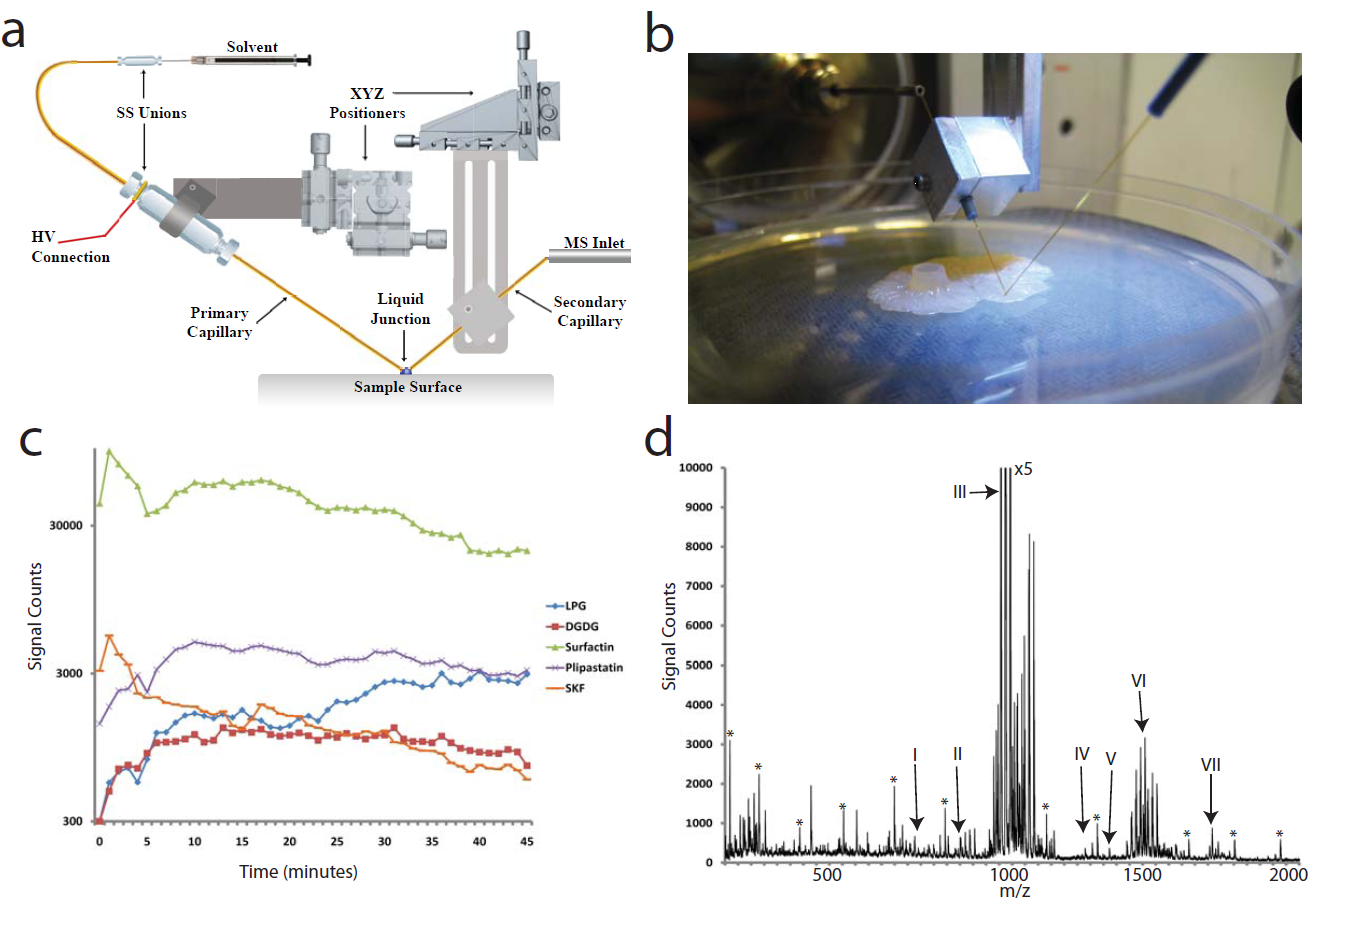
\includegraphics[width=\textwidth]{figures/figNanoDESI.png}
%%    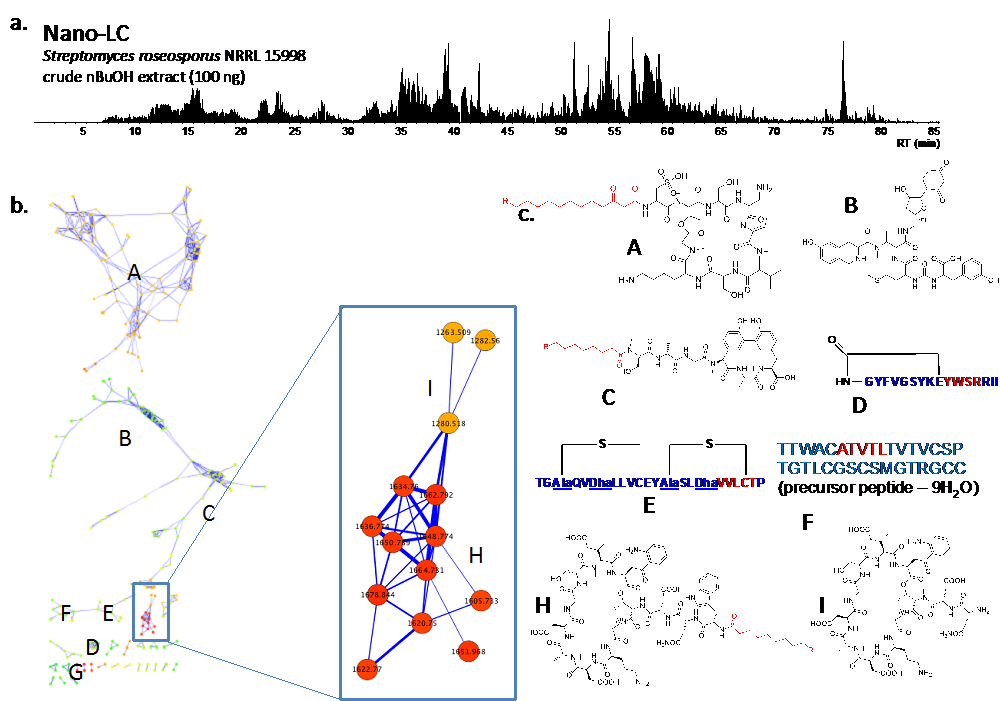
\includegraphics{figures/figApproach.png}
%  \caption{{\bf An overview of nanoDESI with analysis of microbial colonies from a Petri dish.} a) A schematic overview of nanoDESI. HV stands for high voltage. b) A photograph of the nanoDESI set-up with a microbial colony grown on an agar surface in a Petri dish. c) Time dependent analysis at a single location within a 3-day old B. subtilis 3610 colony to indicate the changes in signal intensity of specific molecules over time. Solvent used was methanol:acetonitrile:toluene (50:35:15). d) A mass spectrum obtained from a B. subtilis 3610 colony with nanoDESI. *correspond to agar sugar signals, I is DGDG, II is lysyl-phosphatidylglycerol (LPG,) III is surfactin, IV is sublancin (3+), V is Sporulation killing factor (SKF) (2+), VI is plipastatin, VII is subtilosin (2+).}
%  \label{fig.dbp.dorrestein.desi}
%\end{figure}

%These experiments will utilize a recently developed technology, electron transfer dissociation (ETD), to map the major disulfide cross-links occurring in oxidized and aggregated crystallins from cataractous human lenses.  This robust method takes advantage of the ability of a mobile electron transferred to a peptide in the gas phase within a mass spectrometer to specifically break disulfide bonds so that cross-linked peptides can be identified (21, 22).

HMW aggregates and WI proteins from age-matched control and cataractous lenses will be processed to avoid artifactual oxidation or disulfide exchange reactions during sample preparation by inclusion of iodoacetamide during lens homogenation.  Appropriate techniques will then be used to isolate cross-linked crystallins by de-aggregating lens HMW and WI proteins using guanidine-HCl followed by gel filtration to isolate the cross-linked species that elute before the major peak of crystallin monomers at approximately 25kDa. These cross-linked peptides will then be digested using a combination of LysC and trypsin (and possibly other enzymes, as determined in consultation with CCMS) and the resulting peptides separated by cation-exchange chromatography. % This will further purify disulfide-linked peptides due to their greater net positive charge compared to other peptides. At pH 3, disulfide cross-linked peptides have a net charge of at least +4 due to the presence of two tryptic termini and two N-termini.
%
Disulfide linked peptides and chemically induced cross-linked will be separated by reverse phase chromatography and analyzed using an LTQ/ETD Velos linear ion trap and an LTQ/ETD Elite Orbitrap.  The instruments will be configured to cycle through single MS scans to identify highly-charged precursor peptides for further analysis, followed by 6 data-dependant MS/MS scans, which will be acquired using either CID, HCD or ETD MS/MS. Data acquired using CID/HCD MS/MS will be processed using CCMS UniLink (described in TRD4) for identification of paired disulfide-linked peptides. In addition, ETD MS/MS will be used to fragment disulfide bonds and liberate the individual cross-linked peptides so that they can be sequenced in the following additional 5 data-dependant MS/MS/MS scans. During these MS/MS/MS scans the liberated peptides from the cross-linked species will be fragmented by collision-induced dissociation (CID) to generate typical y and b ions (see Figure~\ref{fig.dbp.david.etd}).

\begin{figure}[htb!]
%  \vspace{-20mm}
    \centering
    \includegraphics[width=0.9\textwidth]{figures/figDbpDavidETD.pdf}
  \caption{\footnotesize {\bf Identification of a disulfide-bridged peptide pair} between $\gamma s$-crystalin and $\beta A3$-crystalin in WI protein from the nucleus of a 93-year-old donor with severe age-related +4 nuclear cataract.  % The data comes from a late eluting cation exchange fraction that was then separated by reverse phase chromatography and analyzed to detect disulfide-linked peptides as described above.  %The MS scan shown in (A) was collected at 52 min during the reverse phase separation and contains many coeluting peptides.
  (A) A peptide at m/z = 502.3 triggered a cycle of 6 data-dependant scans, the first one being the MS2 spectrum shown in (B) where the peptide seen at m/z 502.3 was fragmented using ETD.  The major species in this spectrum is the unfragmented parent ion at m/z = 502.3. % This is a major ion in the spectrum because electron transfer during ETD is relatively inefficient.
  The second and third most abundant ions in this spectrum are two fragment ions at m/z = 358.6 and 896.2, which were selected % for MS/MS/MS.  The instruments control software automatically initiated MS3 scans using CID to fragment these m/z 358.6 and 896.2 ions
  to yield the two MS/MS/MS spectra shown in (C) and (D).  The m/z ion at 896.2 was identified as the doubly charged ion of peptide 163-177 from $\beta A3$-crystallin, and the peptide at m/z 358.6 was identified as the doubly charged peptide 126-131 from $\gamma s$-crystallin.  %The mass of the original disulfide linked peptide was calculated to be 2503.2.  The +5, +4 and +3 charge states of this disulfide linked peptide would be m/z = 501.6, 626.8, and 835.4, respectively.
  }
  \label{fig.dbp.david.etd}
\end{figure}

Samples of HMW, WS and WI proteins from age matched normal lenses and lenses from donors with increasing severity of age-related nuclear cataract will be cross-linked using DTSSP. The nearest neighbors in each of the three lens fractions will be determined by the frequency of identified cross-links between various crystallin subunits, and the contact sites between individual molecules will be mapped.  These results will be compared to cross-linking data produced from purified oligomeric crystallins, and the reported structures, if available, to assess whether the crystallins in the WS, HMW, and WI fractions possess different oligomeric structures than purified crystalliins.  For example, $\beta$-crystallins may have different preferred binding partners in the HMW and WI fractions than they do in either the purified state or in the WS fraction.  We will compare the cross-linking results from normal and cataractous lenses to determine if the organization of the HMW and WI proteins are altered in cataract.  This will test the hypothesis that the WI protein in normal lenses possesses the same oligomeric structure as the HMW fraction, but is altered during cataract formation by new interactions stabilized by disulfide bonding instead of interactions resulting from binding to $\alpha$-crystallins as in normal lenses.   Since there is some evidence that WI crystallins in aged lenses may adopt a fibrillar structure, we will also produce fibrillar aggregates in vitro using purified crystallins and subject them to cross-linking.  The pattern of cross-linking in these fibrillar structures will then be compared to the cross-linking found in naturally occurring crystallin aggregates.  For DTSSP experiments, the disulfide bond in the chemical cross-linker will instead be fragmented by ETD to release the two cross-linked peptides.  Once separated, each of the released peptides will be identified using MS/MS/MS scans as before. The only difference for DTSSP cross-linked peptides will be that Lysine residues will have a 88~Da mass increase due to the attachment of the cleaved spacer. Since the DTSSP reagent is symmetrical, both cross-linked lysine residues in the liberated peptides will undergo the same 88~Da mass increase, and will be identified by their appearance in at least 2 out of the 5 consecutive data-dependant MS3 scans following cleavage of the disulfide bond by ETD.

In collaboration with CCMS, these CID MS/MS/MS spectra will be searched using CCMS spectral library (TRD3) and database (TRD4) search algorithms to identify the individual cross-linked peptides. Spectral library searches will be conducted using the spectral libraries derived from the Lens Atlas proposed above. We note that this enables the possibility of identifying disulfide-linked ultramodified peptides. The spectral alignment, matching and projection algorithms proposed by CCMS are designed to identify spectra that differ by one modification, as would be the case for every Atlas peptide (with alkylated Cysteines) matched to a dissociated MS/MS/MS spectrum (with unalkylated Cysteines). Thus, as soon as a new peptide is added to the Lens Atlas it will also be very likely possible to identify any disulfide-linked version of the same peptide since it will again differ from the MS/MS spectrum by only one modifications (alkylated/unalkylated Cysteine), irrespective of the total number of post-translational modifications per peptide. A similar principle applies to DTSSP cross-linked peptides digested with enzymes other than trypsin or LysC.

\paragraph{Impact of the expertise of the CCMS investigators on DBP.} Drs. Bandeira and Pevzner were the original proponents of the spectral networks paradigm for analysis of peptide MS/MS spectra, including the first application of spectral networks for discovery of post-translational modifications (PTMs), which was demonstrated by analyzing cataractous lens proteomics data~\cite{bandeira07pnas}. Spectral networks algorithms have been extended since then and applied to other analysis of PTMs. In addition, Drs. Bafna, Bandeira and Pevzner also led the development of algorithmic approaches for spectral library search~\cite{wang10} and analysis of PTMs~\cite{tsur05,na11}, including direct collaborations~\cite{Wilmarth06,tanner08} with Dr. David on the analysis of cataractous lens proteomics. Dr. Bandeira also led the development of the ProteoSAFe platform which already enabled the analysis of over 1 billion spectra and thus has the required expertise to implement, search and distribute the proposed Lens Atlas.

%{\bf Application.} The methodology will be used to identify the major disulfide linked peptides in the HMW and WI proteins of cataractous human lenses.  Negative controls in these experiments will consist of normal age-matched lenses or lenses from young donors that do not contain oxidized disulfides.  Distances between disulfide cross-linked cysteine residues in known crystallin structures will be calculated using DS ViewerPro software (Accelrys Inc.) to determine if the observed cross-link is compatible with the predicted structure of the crystallin. In cases where there are no expected interactions, such as in the  A3 and  S cross-link described above, the surface accessibility of the participating cysteines will be calculated to see if they are surface exposed or buried in the predicted structure.  Cross-linking of buried residues would be expected if the crystallin is unfolded. The sensitivity of the procedure may also allow detection of disulfide cross-links between crystallins and non-crystallins, such as membrane proteins that may also be important in the aggregation process (37).  These studies of human lens will also be performed in parallel with the analysis of disulfide cross-links in crystallns from guinea pigs with hyperbaric oxygen induced cataracts during our collaboration with Dr. Frank Giblin.  This will be an important test of the relevance of his unique animal model of age-related human cataract.

%Cross-linking of HMW, WS, and WI crystallins from aged and cataractous human lens.  Following the preliminary experiments described above, samples of HMW, WS and WI proteins from age matched normal lenses and lenses from donors with increasing severity of age-related nuclear cataract will be cross-linked using DTSSP, the cross-linked peptides from intermolecular cross-linked species isolated by gel filtration under denaturing conditions, cross-linked peptides purified by cation-exchange as described in aim 2, and the cross-links identified by mass spectrometry using the ETD based approach.  The nearest neighbors in each of the three lens fractions will be determined by the frequency of identified cross-links between various crystallin subunits, and the contact sites between individual molecules will be mapped.  These results will be compared to cross-linking data produced from purified oligomeric crystallins, and the reported structures, if available, to assess whether the crystallins in the WS, HMW, and WI fractions possess different oligomeric structures than purified crystalliins.  For example, $\beta$-crystallins may have different preferred binding partners in the HMW and WI fractions than they do in either the purified state or in the WS fraction.  We will compare the cross-linking results from normal and cataractous lenses to determine if the organization of the HMW and WI proteins are altered in cataract.  This will test our hypothesis that the WI protein in normal lenses possesses the same oligomeric structure as the HMW fraction, but is altered during cataract formation by new interactions stabilized by disulfide bonding instead of interactions resulting from binding to $\alpha$-crystallins as in normal lenses.   Since there is some evidence that WI crystallins in aged lenses may adopt a fibrillar structure, we will also produce fibrillar aggregates in vitro using purified crystallins and subject them to cross-linking.  The pattern of cross-linking in these fibrillar structures will then be compared to the cross-linking found in naturally occurring crystallin aggregates.  We hypothesize that the WI material in lens is predominately amorphous in nature, but composed of assembles of crystallin aggregates characterized by specific molecular contacts, and that these contacts differ from those found in fibrils.


%%**************************************************************************************
%% ------------------------------------------------------------------------------------
%\section{Technology Research and Development projects (TR\&Ds)}
%% ------------------------------------------------------------------------------------
%%**************************************************************************************
%

% For all 3 aims

%\bibliographystyle{plain}
\bibliographystyle{plain}
\bibliography{../../bibtex/msms,../../bibtex/bandeiraLab,../../bibtex/immunology}
\end{document}
